\section{Heart model}
\label{sec:heartcellularautomata}
For the verification of \acp{ICD},
we adopt the \acf{CA}-based heart model developed in \cite{Spector11_Emergence},\cite{CorreaEtAl11_EGMFractionation}.
%Like \cite{BartocciCBESG09_HIOAmodeling}, it is based on \acf{CA} and is augmented with differential equations in each cell to describe the evolution of the transmembrane voltage with time.
This model lies in-between high spatial fidelity but slow to compute PDE-based whole heart models, and low spatial fidelity but very fast-to-compute automata-based models \cite{TECS}.
PDE-based models and ionic currents \cite{Islam1MGSG14_CompositionalityCells} may be more accurate but are not currently amenable to formal verification.
\ac{CA}-based models were used in \cite{BartocciCBESG09_HIOAmodeling} and \cite{Chen14_Quantitative}.
This paper's model also has the important advantage of forming the basis of software used to train electrophysiologists, and allows interactive simulation of surgical procedures like ablation \cite{visibleep}.
\yhl{In particular, it can simulate tachycardias.}%

\textbf{This paper's automata:} All hybrid automata in this paper have the whole state space as invariants and transitions are urgent (taken immediately when the guard is enabled).
The \ac{EGM} voltage signal $\egm$ has upper and lower bounds.
We also observe that, as will be seen in Section \ref{sec:discriminators},
i) the \ac{ICD} will always reach a decision of VT or SVT in finite time, 
ii) at which point it resets its \yhl{controlled (software) variables} so new values are computed for the next arrhythmia episode.
So while the heart can beat indefinitely, for the purposes of \ac{ICD} verification, 
there's a uniform upper bound on the length of time of any execution.
Let $D \geq 0$ be this duration ($D$ is on the order of 30sec depending on device settings).
\yhl{Therefore, every mode of every automaton in what follows has a transition to mode End in which time does not progress.
We don't show these transitions in the automata figures to avoid congestion.
}

\subsection{Cellular automata model}
The heart has two upper chambers called the \emph{atria} and two lower chambers called the \emph{ventricles} (Fig. \ref{fig:icd})
The synchronized contractions of the heart are driven by electrical activity.
Under normal conditions, the SinoAtrial (SA) node (a tissue in the right atrium) spontaneously \emph{depolarizes}, producing an electrical wave that propagates to the atria and then down to the ventricles (Fig.\ref{fig:overview})
In this model, the myocardium (heart's muscle) is treated as a 2D surface (so it has no depth), and discretized into \emph{cells}, which are simply regions of the myocardium (Fig. \ref{fig:overview}). 
Thus we end up with $N^2$ cells in a square $N$-by-$N$ grid.
A cell's voltage changes in reaction to current flow from neighboring cells, and in response to its own ion movements across the cell membrane.
This results in an \emph{\ac{AP}}.

Fig. \ref{fig:cellaut} shows how the \ac{AP} is generated by a given cell \cite{Klabunde_CVEPconcepts}:
in its quiescent mode (Phase 4), a cell $(i,j)$ in the grid has a cross-membrane voltage $V(i,j,t)$ equal to $V_{min} < 0$.
As it gathers charge, $V(i,j,t)$  increases until it exceeds a threshold voltage $V_{th}$.
\yhl{In Phase 0}, the voltage then experiences a very fast increase (Phase 0), called the upstroke, to a level $V_{max} > 0$, after which it decreases \yhl{(Phase 1)} to a plateau \yhl{(Phase 2)}.
It stays at the plateau level for a certain amount of time \textbf{PD} then decreases linearly to below $V_{th}$ (Phase 3 - ERP).
Once below $V_{th}$ it is said to be in the Relative Refractory Period (Phase 3 - RRP) .
\yhl{In Phase 3 - RRP}, the cell can be depolarized a second time, albeit at a higher threshold $V_{th,2}$, slower and to a lower plateau level $V_{max,2} < V_{max}$ \yhl{(Upstroke 2)}.
Otherwise, when the voltage reaches $V_{min}$ again, the cell enters the quiescent stage again. 
This model is suitable for both pacemaker and non-pacemaker cells, the main differences being in the duration of the plateau (virtually non-existent for pacemaker cells), and the duration of phases 0 and 4 (both are shorter for pacemaker cells).

In Fig. \ref{fig:cellaut}, $V(i,j) \in \Re$ denotes the voltage in cell $(i,j)$ of the grid, and \yhl{$V =(V(1,1),\ldots, V(N^2,N^2))^T$} in $\Re^{N^2}$ groups the cross-membrane voltages of all cells in the heart.
The whole heart model $\Sys_{CA}$ is the parallel composition of these $N^2$ single-cell models. 
\begin{figure}[t]
	\centering
	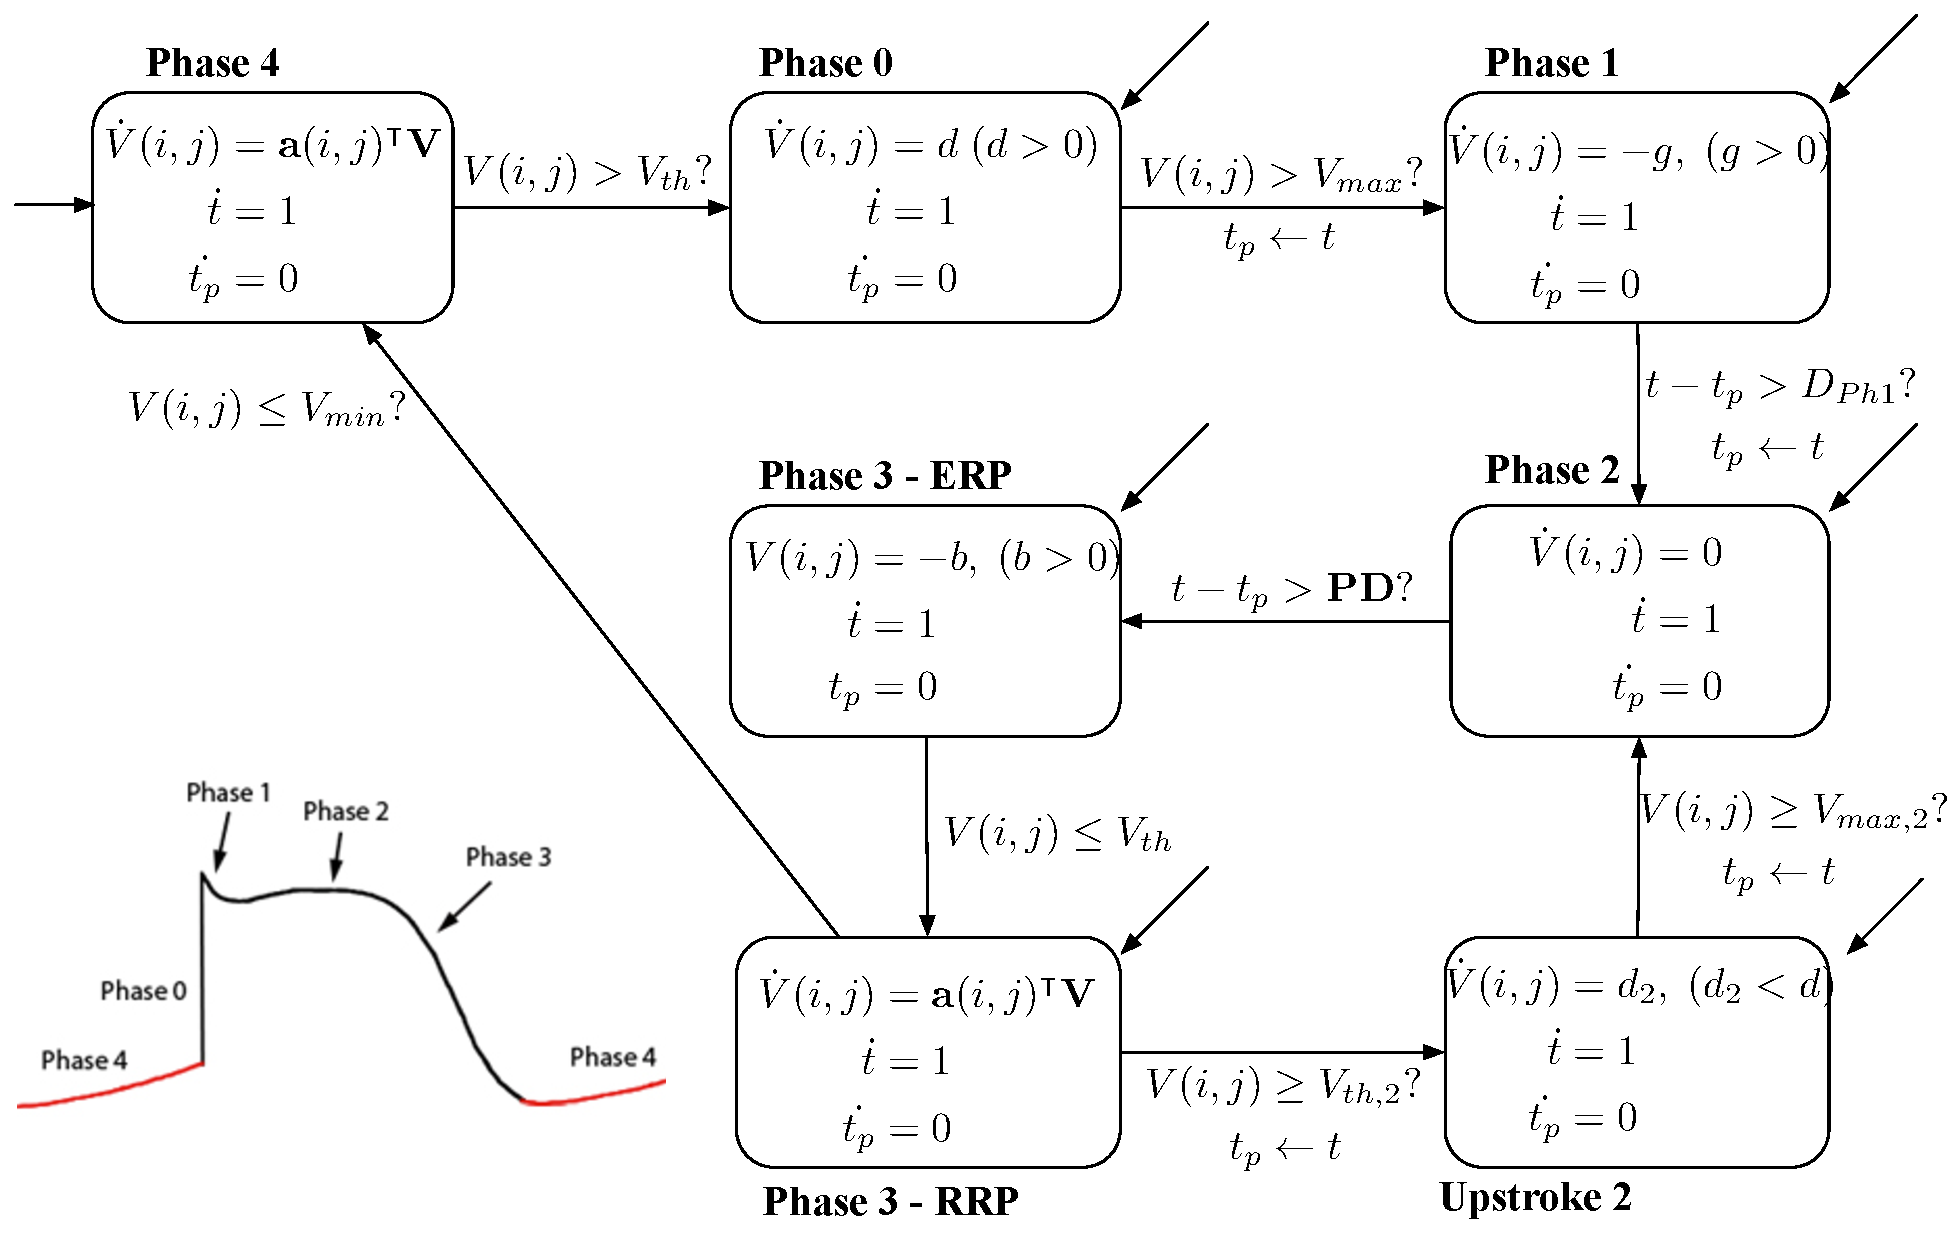
\includegraphics[scale=0.26]{figures/cellaut1v2}
	\vspace{-10pt}
	\caption{Hybrid model $\Sys_c$ of one cell of the heart model. AP figure from \cite{eplab}. 
		$V_{th,2}>V_{th}$, $V_{max,2}<V_{max}$}
	\vspace{-20pt}
	\label{fig:cellaut}
\end{figure}
%
The $(i,j)^{th}$ cell's voltage at time $t$ in Phase 4 depends on that of its neighbors and its own as follows \cite{Spector11_Emergence}
\begin{eqnarray}
\dot{V}(i,j,t) &=& \frac{1}{R_h(i,j)}[V(i-1,j,t)+V(i+1,j,t) - 2V(i,j,t)] 
\nonumber \\ 
&& +  \frac{1}{R_v(i,j)}[V(i,j-1,t) +  V(i,j+1,t) - 2V(i,j,t)]  
\nonumber\\
&=& a(i,j)^TV(t), \; a(i,j) \in \Re^{N^2}
\;
\end{eqnarray}
where $R_h$, $R_v$ are conduction constants that can vary across the myocardium.
Thus $V$ evolves according to a linear ODE $\dot{V} = AV$ where $A$ is the matrix whose rows are the $a(i,j)$. 
The two states $t$ and $t_p$ are clocks.
Clock $t_{p}$ keeps track of the value of the last discrete jump. 
We will use this arrangement in all our models: it avoids resetting the clocks which preserves Reset Monotonicity.

\acp{ICD} observe the electrical activity through three channels (Fig.~\ref{fig:icd}).
Each signal is called an \acf{EGM} signal.
The signal read on a channel is given by \cite{CorreaEtAl11_EGMFractionation}:
\begin{equation}
	\label{eq:vegm}
	\egm(t) = \frac{1}{K} \sum_{i,j} \left(\frac{1}{||p_{i,j}-p_0|| } - \frac{1}{||p_{i,j}-p_1||}\right) \dot{V}(i,j,t)
\end{equation}
\yhl{where $\|\cdot\|$ is the Euclidian norm, $p_0$ and $p_1$ are the electrodes' positions and $p_{i,j}$ is the position of the $(i,j)^{th}$ cell on the 2D myocardium ($p_0,p_1,p_{i,j} \in \Re^2$). 
Positions $p_0,p_1$ should be chosen different from $p_{i,j}$ to avoid infinities.}
%This model was validated against real recordings in vitro \cite{StinnettDonnelly12_EGMresolution}.

\textbf{Extensions}. 
The Action Potential Duration (APD) restitution mechanism as modeled in \cite{Spector11_Emergence} can be included in this model without changing its formal properties.

We now state the main result of this section.
\begin{thm}
	\label{thm:heartCA}
	Let $\Sys_{CA}$ be the whole heart cellular automaton model obtained by parallel composition of $N^2$ models $\Sys_c$ with state vector $x = [V, t,t_p,\egm ] \in \Re^{N^2}\times \Re^{3}$.
	Assume that all executions of the system have a duration of $D\geq 0$.
	Then $\Sys_{CA}$ is STORMED.
\end{thm}